\documentclass[aspectratio=169,kulak,t,handout]{kulakbeamer} % handout

\usepackage{tikz}
\usetikzlibrary{positioning}
\usepackage{hyperref}
\usepackage[dutch]{babel}
\usepackage[T1]{fontenc}
\usefonttheme[onlymath]{serif}

\title[Groep 1 - Safety First]{Miniatuurrobotwagen in een Smart City}
\subtitle{Probleemoplossen en ontwerpen, deel 2}
\author{Camille Louagie, Emiel Vanspranghels, Otto Meerschman, Ruben Leenknecht, Staf Rys}
 
\institute[Kulak]{KU Leuven Kulak}
\date{Academiejaar 2020 -- 2021}

\AtBeginSection[]{\only<beamer>{\addtocounter{framenumber}{-1}
		\begin{outlineframe}\frametitle{Overzicht}
			\tableofcontents[currentsection,hideallsubsections]
	\end{outlineframe}}}

\linespread{1.2}
\begin{document}

\begin{titleframe}
\titlepage
\end{titleframe}


\section*{Probleemstelling en oplossing}

\begin{frame}
	\frametitle{{\Large Verdere verstedelijking creëert mobiliteitsproblemen.}}


	\begin{figure}
		\centering
		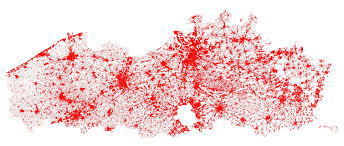
\includegraphics[width=.6\textwidth]{ruimtelijkestaat}
		%rood= ruimtebeslag > drempelwaarde
		
		\label{fig:ruimtelijkestaat}
	\end{figure}
\end{frame}

\begin{frame}
	\frametitle{{\large Slimme steden als oplossing voor het mobiliteitsprobleem}}
	
\begin{block}{Definitie}
	
	Een stad die technologische innovatie gebruikt om de stedelijke werking efficiënt te laten verlopen
	
\end{block}	
	\begin{itemize}
		\large\item  Verbeteren van interacties
		\begin{itemize}
			\normalsize\item Fysieke beperkingen
			\item Levenskwaliteit verhogen
		\end{itemize}
		\item  Diensten vereenvoudigen
	\end{itemize}
\end{frame}



\begin{frame}{{\Large Wegen de voordelen van zelfrijdende auto's op tegen de nadelen?}}
	\begin{columns}
	\column{0.5\textwidth}\centering
	{\bf{Voordelen}}\\[.2cm]

		\begin{itemize}
			\large\item Rijden nauwkeuriger
			\begin{itemize}
				\normalsize\item Meer parkeerplaatsen
				\item Minder files
			\end{itemize}
			\item Respect voor verkeersregels
			
		\end{itemize}
	\column{0.5\textwidth}\centering
	{\bf{Nadelen}}\\[.2cm]

			\begin{itemize}
			\large\item Kwetsbaar voor hackers
			\item Daling overheidsinkomsten
			\item Stijging werkeloosheid
			\end{itemize}
	
	\end{columns}
\end{frame}

\begin{outlineframe}[Overzicht]
	\tableofcontents
\end{outlineframe}


\section{Schets van de situatie}

\begin{frame}{Negen kruispunten vormen een modelstad.}
	
	\begin{tikzpicture}
		\node [anchor=west] (Volglijn met stopstreep) at (-2,0.8) {\Large Volglijn met stopstreep};
		\node [anchor=west] (verkeerslicht) at (-2,2.5) {\Large Verkeerslicht};
		
		\node [anchor=west] (Weg) at (11,3.2)[red] {\large 250 mm};
		\begin{scope}[xshift=1.5cm]
			\node[anchor=south west,inner sep=0] (image) at (2,0) {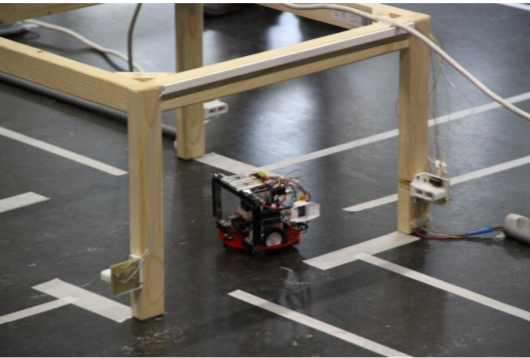
\includegraphics[width=0.5\textwidth]{modelstad}};
			\node [anchor=west] (Afstand) at (8.5,2.0)[red] {\large 75 mm};
			\begin{scope}[x={(image.south east)},y={(image.north west)}]
				%\draw[cyan,ultra thick,rounded corners] (0.4,0.55) rectangle (0.2,0.3);
				\draw [-stealth, line width=3pt, cyan] (Volglijn met stopstreep) -- ++(0.43,0.0);
				%\draw[cyan,ultra thick,rounded corners] (0.4,0.55) rectangle (0.2,0.3);
				\draw [-stealth, line width=3pt, cyan] (verkeerslicht) -- ++(1.05,0.0);
			\end{scope}
				\draw[thick,red,->,line width=0.5mm] (8.5,1.65) -- (8.5,2.5);
				\draw[thick,red,->,line width=0.5mm] (8.5,2.5) -- (8.5,1.65);
				\draw[thick,red,->,line width=0.5mm] (9.5,2.7) -- (9.5,3.65);
				\draw[thick,red,->,line width=0.5mm] (9.5,3.65) -- (9.5,2.7);
		\end{scope}
	\end{tikzpicture}
\end{frame}






\section{Robot hardware}

\begin{frame}{Ontwerp}
\noindent
\begin{tikzpicture}
	\node [anchor=west] (Batterij) at (-2,4) {\Large Batterij};
	\node [anchor=west] (Kleurensensor) at (-2,5.5) {\Large Kleurensensor};
	\node [anchor=west] (Afstandssensor) at (-2,1) {\Large Afstandssensor};
	\node [anchor=west] (Microcontroller) at (-2,3) {\Large Microcontroller};
	\begin{scope}[xshift=1.5cm]
		\node[anchor=south west,inner sep=0] (image) at (0,0) {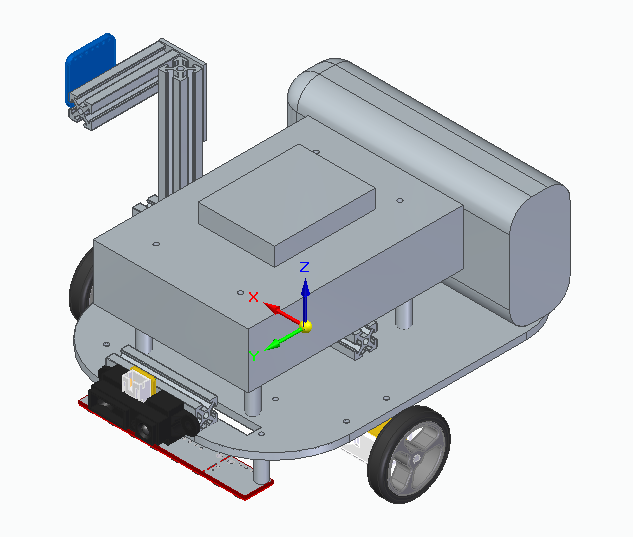
\includegraphics[width=0.5\textwidth]{afbchassis}};
		\begin{scope}[x={(image.south east)},y={(image.north west)}]
			%\draw[cyan,ultra thick,rounded corners] (0.4,0.55) rectangle (0.2,0.3);
			\draw [-stealth, line width=3pt, cyan] (Batterij) -- ++(1.1,0.0);
			%\draw[cyan,ultra thick,rounded corners] (0.4,0.55) rectangle (0.2,0.3);
			\draw [-stealth, line width=3pt, cyan] (Kleurensensor) -- ++(0.4,0.0);
			\draw [-stealth, line width=3pt, cyan] (Afstandssensor) -- ++(0.4,0.1);
			\draw [-stealth, line width=3pt, cyan] (Microcontroller) -- ++(0.4,0.0);
		\end{scope}
	\end{scope}
\end{tikzpicture}
\end{frame}


\begin{frame}
\noindent
\begin{tikzpicture}
	\node [anchor=west] (Kogelrol) at (-1,3) {\Large Kogelrol};
	\node [anchor=west] (Lijnsensor) at (-1,2) {\Large Lijnsensor};
	\node [anchor=west] (Wiel) at (-1,0) {\Large Wiel};
	\begin{scope}[xshift=1.5cm]
		\node[anchor=south west,inner sep=0] (image) at (0,0) {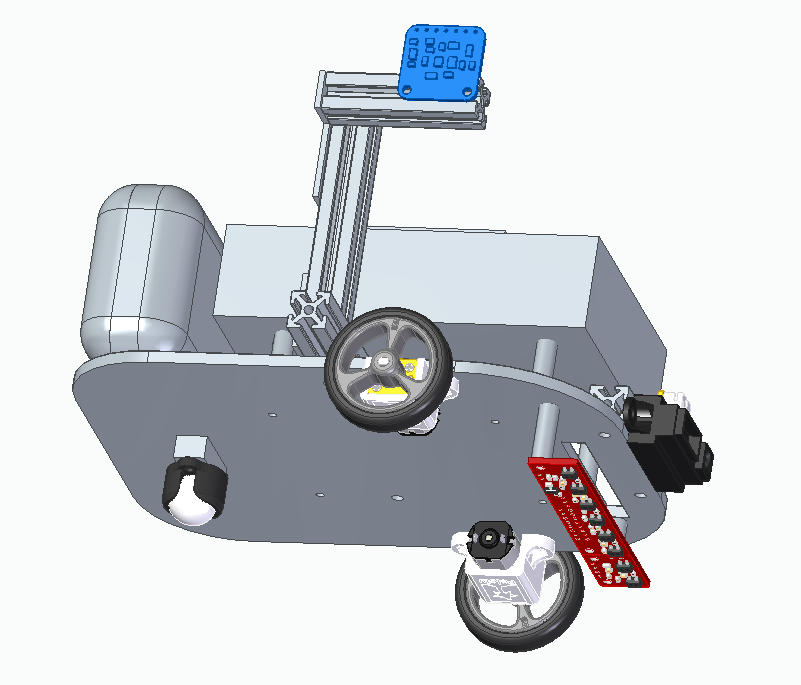
\includegraphics[width=0.6\textwidth]{OAZ}};
		\begin{scope}[x={(image.south east)},y={(image.north west)}]
			%\draw[cyan,ultra thick,rounded corners] (0.4,0.55) rectangle (0.2,0.3);
			\draw [-stealth, line width=3pt, cyan] (Kogelrol) -- ++(0.45,0.0);
			%\draw[cyan,ultra thick,rounded corners] (0.4,0.55) rectangle (0.2,0.3);
			\draw [-stealth, line width=3pt, cyan] (Lijnsensor) -- ++(0.8,0.0);
			\draw [-stealth, line width=3pt, cyan] (Wiel) -- ++(0.6,0.1);
		\end{scope}
	\end{scope}
\end{tikzpicture}	
\end{frame}

\begin{frame}{Keuzes bij het zelfontworpen chassis}
	\begin{columns}
	\begin{column}{0.50\textwidth}\centering
		%{\bf{Onderdelen}}\\[.2cm]
		\begin{itemize}
			\Large\item Afmetingen
			\item Hoek met de grond
			\item Lijnsensor
			\item Wielen
		\end{itemize}
	\end{column}
	\begin{column}{0.75\textwidth}\centering
		{\bf{Chassis-model}}\\[.2cm]
		\begin{figure}
			\centering
			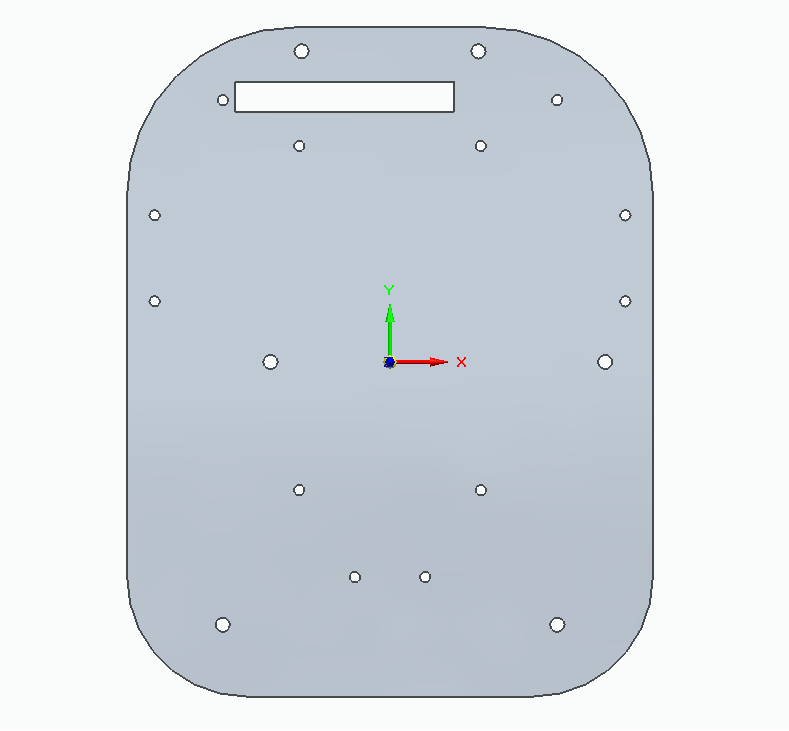
\includegraphics[width=.55\textwidth]{chassis3d}
			
			\label{fig:chassis}
		\end{figure}
	\end{column}
\end{columns}	
\end{frame}

\section*{Besluit}






\begin{frame}{Besluit}
\begin{itemize}
	\large \item Zelfrijdend wagentje: Legt probleemloos een parcours af
	\item Toont mogelijkheden op grote schaal
	\item Budgetoverschot: Veiling anders aanpakken
	
\end{itemize}	
	
\end{frame}





	
\section{Referenties}

\begin{frame}[allowframebreaks]
	\frametitle{References}
	\nocite{*}
	\bibliographystyle{amsalpha}
	\bibliography{bibliografietv.bib}
\end{frame}

\end{document}